\chapter{Results}

\section{Correlation analysis}

\subsection{Bivariate correlations}

\begin{figure}[htbp]
    \caption{Correlation matrix}
    \centering
    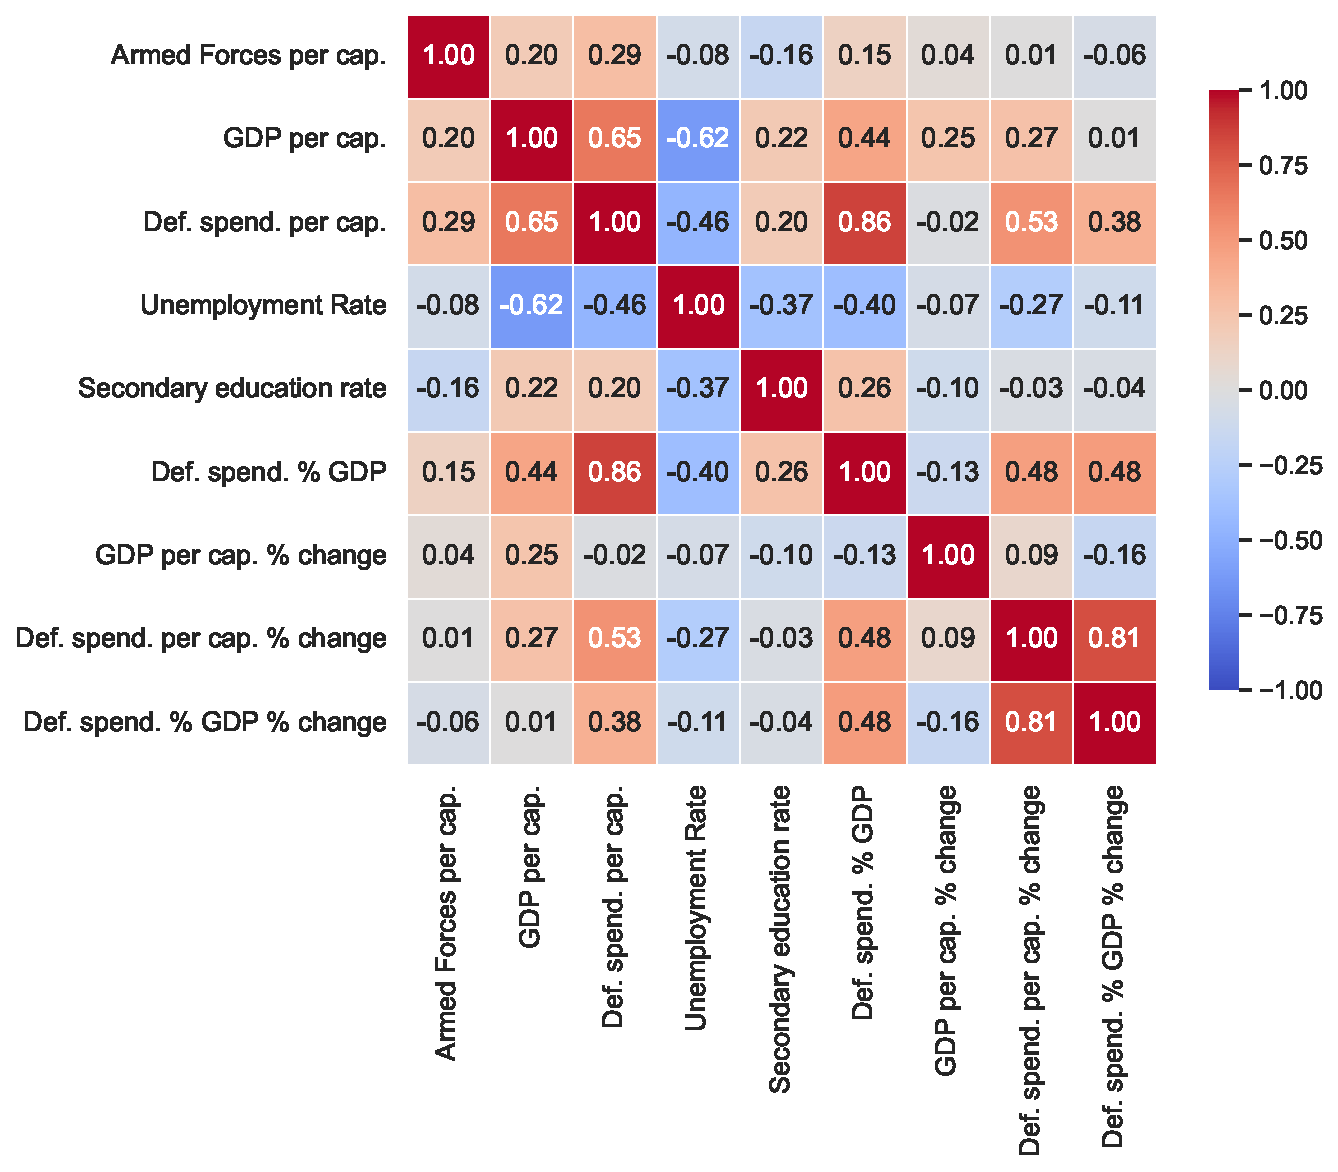
\includegraphics[width=1\textwidth]{images/correlation_heatmap.pdf}
    \label{fig:correlation_heatmap}
\end{figure}

As shown in Figure~\ref{fig:correlation_heatmap}, the correlation analysis revealed no single factor with a strong correlation to active military personnel numbers.
Active armed forces per capita were found to have weak to moderate positive correlations with GDP per capita (0.17), defence spending proportion of GDP (0.14) and defence spending per capita (0.29).
Weak negative correlations were observed with unemployment rate (-0.08), secondary education attainment rate (-0.12) and defence spending proportion of GDP annual change (-0.11). 
These findings suggest that military size may grow as a country's economy improves and defence spending rises, while higher unemployment and education attainment rates may be related to reductions in military personnel.

GDP per capita and unemployment rate exhibited a moderate negative correlation (-0.62), which could indicate that a stronger economy is associated with better labour market conditions. 
Even stronger correlations were found between defence expenditure per capita and defence expenditure's proportion of GDP (0.85), and between their annual changes (0.80). 
This was unsurprising given that these variables are derived from defence spending. 
However, such large correlations may indicate multicollinearity, which could bias regression estimates and inflate standard errors. 
This meant that multicollinearity should be 
assessed before running the regression.

While the correlation analysis provides useful preliminary insight into the relationships between the variables, it does not isolate the direct effect of each variable. 
Therefore, a fixed-effects regression is used to estimate the conditional effects of the economic variables on active armed forces per capita, controlling for unobserved time-invariant heterogeneity across countries.

\subsection{Multicollinearity}

\begin{table}[ht]
\caption{Variance Inflation Factors (all variables)}
\small
\centering
\begin{tabularx}{\textwidth}{l r}
\toprule
\textbf{Variable} & \textbf{VIF} \\
\midrule
Unemployment rate & 1.95 \\
Secondary education rate & 1.27 \\
GDP per capita & 2.73 \\
Defence spending per capita & 6.00 \\
Defence spending \% of GDP & 4.93 \\
GDP per capita \% change & 1.35 \\
Defence spending per capita \% change & 4.28 \\
Defence spending \% GDP \% change & 4.43 \\
\bottomrule
\end{tabularx}
\label{tab:multicollinearity_full}
\end{table}

The initial results, displayed in Table~\ref{tab:multicollinearity_full}, showed moderate to high VIFs for defence spending per capita (6.00), defence spending as a percentage of GDP (4.93) and their respective annual percentage changes (4.28 and 4.43), indicating the presence of multicollinearity. 
This is expected as these variables were highly correlated and capture similar underlying dynamics.
To mitigate this, the variables defence spending per capita and its annual change were removed, and VIF values were calculated again.
It should be noted that a high VIF does not always justify the elimination of a variable; the exclusion should be theoretically motivated, for example, if two variables measure the same underlying factor \parencite{obrien_caution_2007}. 
In this case, the exclusion makes sense, as the two defence spending variables and their annual changes are conceptually similar.

Table~\ref{tab:multicollinearity_reduced} reports the VIF values, excluding the possibly multicollinear variables.
The VIF values reduced significantly, with defence spending's share of GDP now having 1.93 and its annual change having 1.50. 
The observed reduction in multicollinearity motivated the estimation of two regression models: a full model including all variables and a reduced model excluding the highly collinear variables.
These models can then be used for a robustness check to ensure whether the findings of the models are stable or influenced by multicollinearity.

\begin{table}[ht]
\caption{Variance Inflation Factors (reduced variables)}
\small
\centering
\begin{tabularx}{\textwidth}{l r}
\toprule
\textbf{Variable} & \textbf{VIF} \\
\midrule
Unemployment rate & 1.89 \\
Secondary education rate & 1.23 \\
GDP per capita & 2.10 \\
Defence spending \% of GDP & 1.93 \\
GDP per capita \% change & 1.19 \\
Defence spending \% GDP \% change & 1.50 \\
\bottomrule
\end{tabularx}
\label{tab:multicollinearity_reduced}
\end{table}

\section{Regression modelling}

\subsection{Robustness check}

Two fixed-effects regression models were estimated to assess the robustness of the model; Table~\ref{tab:robustness} reports their summaries. 
The first was a base model, which included all variables, and the second was a reduced model with defence budget per capita and its annual change excluded, as these variables had exhibited multicollinearity with the defence budget's proportion of GDP and its annual change.

\renewcommand{\arraystretch}{1.3}

\begin{table}[ht]
\small
\caption{Robustness check}
\centering
\resizebox{\textwidth}{!}{%
\begin{tabularx}{\textwidth}{>{\hsize=0.85\hsize\raggedright\arraybackslash}X 
                            >{\hsize=1\hsize\raggedright\arraybackslash}X 
                            >{\hsize=1\hsize\raggedright\arraybackslash}X}
\toprule
\textbf{Term} & \textbf{Base model} & \textbf{Reduced model} \\
\midrule
\multicolumn{3}{l}{\textit{Coefficient estimates}} \\
Unemployment rate & $-0.0108, p=0.3263$ & $-0.0097, p=0.4007$ \\
Secondary education attainment rate & $-0.0062, p=0.0477$ & $-0.0070, p=0.0408$ \\
GDP per capita & $0.3754, p=0.1189$ & $0.8725, p=0.0033$ \\
Def. spend. per capita & $0.3635, p=0.0003$ & - \\
Def. spend. \% GDP & $-0.0984, p=0.0898$ & $0.0918, p=0.0442$ \\
GDP per capita \% change & $-0.0032, p=0.4352$ & $-0.0073, p=0.0989$ \\
Def. spend. per capita \% change & $0.0007, p=0.5899$ & - \\
Def. spend. \% GDP \% change & $-0.0019, p=0.1055$ & $-0.0011, p=0.1599$ \\
\addlinespace
\multicolumn{3}{l}{\textit{Model statistics}} \\
$R^2$ & 0.2820 & 0.2038 \\
F-statistic (robust) & $F(8,237)=4.35, p=0.0001$ & $F(6,239)=2.92, p=0.0091$ \\
\bottomrule
\end{tabularx}
}
\label{tab:robustness}
\end{table}

The base model explained a larger proportion of the variance after accounting for country and year fixed effects $(R^2 = 0.2820\, \text{vs.} \,0.2038)$ and included a statistically significant variable, defence spending per capita, which had a positive relationship with the dependent variable. 
However, the multicollinearity between defence spending per capita and defence spending's share of GDP could undermine the stability and interpretability of the model. 
This was evidenced by the change in the coefficient sign of defence spending's share of GDP from negative to positive. 
That variable was expected to exhibit effects in the same direction as defence spending per capita, as they are derived from the same underlying measure of defence budgets.
The concerns of multicollinearity distorting the model were further supported by the change in significance of GDP per capita, its annual change, and defence spending's share of GDP.
These inconsistencies supported the decision to remove the collinear variables and favour the reduced model, which could be more stable and interpretable.

\subsection{Sensitivity analysis}

Table~\ref{tab:sensitivity} shows the three models that were estimated to analyse the effect of interpolated and filled educational attainment values.
The secondary educational attainment rate coefficients stayed consistently negative across models, although in Model B, it became statistically insignificant. 
Additionally, other coefficients also remained similar in magnitude, indicating that the use of interpolated values did not meaningfully distort the relationship with the target variable. 
This was further supported by the fact that the dummy variable for interpolated values in Model C was not statistically significant, suggesting no systematic differences in observations, where the education rate was imputed.
However, Model B showed shifts in significance for other variables, such as defence spending's share of GDP and its annual change, and the overall model lost statistical significance ($F(6,216)=2.0229$, $p=0.0638$).

\renewcommand{\arraystretch}{1.2}

\begin{table}[ht]
\small
\caption{Sensitivity analysis models}
\centering
\resizebox{\textwidth}{!}{%
\begin{tabularx}{\textwidth}{>{\hsize=0.85\hsize\raggedright\arraybackslash}X 
                            >{\hsize=1\hsize\raggedright\arraybackslash}X 
                            >{\hsize=1\hsize\raggedright\arraybackslash}X 
                            >{\hsize=1\hsize\raggedright\arraybackslash}X}
\toprule
\textbf{Term} & \textbf{Model A (full)} & \textbf{Model B (excl. filled)} & \textbf{Model C (full + dummy)} \\
\midrule
\multicolumn{4}{l}{\textit{Coefficient estimates}} \\
Unemployment rate & $-0.0097, p=0.4007$ & $-0.0111, p=0.3499$ & $-0.0097, p=0.3975$ \\
Secondary education attainment rate & $-0.0070, p=0.0408$ & $-0.0052, p=0.1290$ & $-0.0070, p=0.0417$ \\
GDP per capita & $0.8725, p=0.0033$ & $0.8047, p=0.0066$ & $0.8719, p=0.0034$ \\
Def. spend. \% GDP & $0.0918, p=0.0442$ & $0.1058, p=0.0521$ & $0.0915, p=0.0438$ \\
GDP per capita \% change & $-0.0073, p=0.0989$ & $-0.0072, p=0.1098$ & $-0.0072, p=0.1044$ \\
Def. spend. \% GDP \% change & $-0.0011, p=0.1599$ & $-0.0017, p=0.0321$ & $-0.0011, p=0.1592$ \\
Interpolation dummy & - & - & $0.0049, p=0.8935$ \\
\addlinespace
\multicolumn{4}{l}{\textit{Model statistics}} \\
Number of observations & 285 & 262 & 285 \\
$R^2$ & 0.2038 & 0.2000 & 0.2039 \\
F-statistic (robust) & $F(6,239)=2.9221, p=0.0091$ & $F(6,216)=2.0229, p=0.0638$ & $F(7,238)=3.7099, p=0.0008$ \\
\bottomrule
\end{tabularx}
}
\label{tab:sensitivity}
\end{table}

Based on these results, Model C with full data, including interpolated and filled values, and a dummy for flagging imputed values, was chosen as the preferred regression model. 
While imputed data could introduce noise or subtle bias into regression estimates, this did not appear to be the case this time, as the interpolation dummy variable was found to be statistically insignificant. 
Nevertheless, Model C was adopted as it retains the full sample size while explicitly controlling for data quality variation, thereby increasing the robustness of the model.
Furthermore, Model B, which excluded imputed data, was overall statistically insignificant, again supporting the choice of the full sample and appropriate controls.

\subsection{Regression model analysis}

The summary of the selected model specification is reported in Table~\ref{tab:model_summary}.
The selected fixed-effects regression model had a 0.2039 $R^2$, meaning the independent variables explained approximately 20.39\% of the variation in the logarithm of active armed forces per capita after accounting for fixed effects. 
However, the $R^2$ before removing fixed effects was approximately 0.9555, meaning in total the model explained about 95.55\% of the variation in the dependent variable.
The robust F-statistic for the model was $F(7, 238)=3.7099, p=0.0008$, showing joint significance of the independent variables, while adjusting for potential heteroskedasticity.
In other words, after accounting for country and year fixed effects, the included variables jointly have a significant effect on the dependent variable.

\renewcommand{\arraystretch}{1.3}

% Model Summary Table
\begin{table}[htbp]
\caption{Regression Estimation Summary}
\centering
\begin{threeparttable}
\begin{tabularx}{\textwidth}{@{}lX@{}}
\toprule
\textbf{Dep. Variable} & \texttt{Active Armed Forces per capita} \\
\textbf{Estimator} & PanelOLS (from Python library "linearmodels") \\
\textbf{No. Observations} & 285 \\
\textbf{Entities} & 32 \\
\textbf{Time Periods} & 9 \\
\textbf{Cov. Estimator} & Clustered \\
\midrule
\textbf{R-squared} & 0.2039 \\
\textbf{Log-likelihood} & 274.78 \\
\textbf{F-statistic (robust)} & 3.7099 \\
\textbf{P-value (F-stat)} & 0.0008 \\
\textbf{Distribution} & F(7, 238) \\
\midrule
\textbf{F-test for Poolability} & 60.604 \\
\textbf{P-value} & 0.0000 \\
\textbf{Distribution} & F(39, 238) \\
\textbf{Included effects} & Entity, Time \\
\bottomrule
\end{tabularx}
\end{threeparttable}
\label{tab:model_summary}
\end{table} 

Table~\ref{tab:final_model} reports the parameter estimates for the selected model specification. 
Unemployment rate proved to be statistically insignificant $(-0.0097, p=0.3975)$, indicating that it may not substantially affect military labour supply in the sampled country and year subset.
Secondary education attainment rate exhibited a significant, modest negative relationship $(-0.0070, p=0.0417)$ with the dependent variable, meaning for every 1 percentage point increase in secondary education attainment rate, the active military size per capita decreased by approximately 0.70\%.
This negative relationship could be caused by multiple reasons. For example, more educated individuals may consider their opportunities better in the civilian sector, while it could also be that countries with higher educational attainment rates have more technologically advanced armed forces, which require less manpower.

% Parameter Estimates Table
\begin{table}[htbp]
\caption{Parameter Estimates}
\centering
\begin{threeparttable}
\begin{tabularx}{\textwidth}{@{}Xrrrrrr@{}}
\toprule
\textbf{Variable} & \textbf{Coef.} & \textbf{Std. Err.} & \textbf{t-stat} & \textbf{p-value} & \textbf{CI Lower} & \textbf{CI Upper} \\
\midrule
Unemployment rate & -0.0097 & 0.0115 & -0.8476 & 0.3975 & -0.0323 & 0.0129 \\
Secondary education attainment rate & -0.0070 & 0.0034 & -2.0480 & 0.0417 & -0.0137 & -0.0003 \\
GDP per capita & 0.8719 & 0.2950 & 2.9554 & 0.0034 & 0.2907 & 1.4532 \\
Def. spend. \% GDP & 0.0915 & 0.0451 & 2.0268 & 0.0438 & 0.0026 & 0.1804 \\
GDP per capita \% change & -0.0072 & 0.0044 & -1.6302 & 0.1044 & -0.0160 & 0.0015 \\
Def. spend. \% GDP \% change & -0.0011 & 0.0008 & -1.4120 & 0.1592 & -0.0027 & 0.0004 \\
Education Dummy & 0.0049 & 0.0368 & 0.1340 & 0.8935 & -0.0675 & 0.0774 \\
\bottomrule
\end{tabularx}
\end{threeparttable}
\label{tab:final_model}
\end{table}

The logarithm of GDP per capita had a positive and significant relationship $(0.8719, p=0.0034)$ with armed forces per capita, meaning a 1\% increase in GDP per capita was associated with approximately a 0.87\% increase in active military size per capita. 
This means that wealthier countries tend to have larger active militaries, which could be due to their ability to invest more in the defence sector. 
Wealthier countries may also want to maintain a larger military presence to project power and influence globally.
The annual change in GDP per capita was found to be statistically insignificant $(-0.0072, p=0.1044)$, indicating that short-term economic changes might not influence active military personnel size. 

Defence spending's share of GDP, however, exhibited a significant and positive relationship $(0.0915, p=0.0438)$, meaning that for each percentage point increase in defence spending's proportion of GDP, active military size per capita increased approximately 9.15\%.
The annual changes in defence spending's proportion of GDP proved to be an insignificant predictor of active armed forces numbers $(-0.0011, p=0.1592)$. 
These findings could indicate that a higher baseline proportion of defence spending in GDP may signal long-term commitments to maintaining a large military, while short-term changes in the proportion may not directly predict a change in active military personnel. 
It could also be that short-term investments in defence spending were used for assets other than manpower.

It is important to note for the interpretation of these coefficients that the dependent variable was active military size per capita, meaning the coefficients reflect relative changes in active military personnel with respect to population size. 
Assuming a stable population, the reported percentage changes in active military size per capita can also be interpreted as approximate percentage changes in total active military size. 
However, in cases where the population can vary notably, the per capita measure provides a more consistent comparison.